 \documentclass{beamer}
\usetheme{Madrid}

%==========Packages================
\usepackage[utf8]{inputenc}
    \usepackage[T1]{fontenc} 
    \usepackage[francais]{babel}
    \usepackage{amsmath}
    \usepackage{amssymb}
    \usepackage{graphicx}
    \usepackage{color}
    \usepackage{hyperref}
    \usepackage[left=2cm,right=2cm,top=2cm,bottom=2cm]{geometry}
    \usepackage{mathrsfs}
    \usepackage{verbatim}
   %========================================
%=====================================================================================================
\title{Application de chiffrement homomorphe à l'apprentissage automatique}
    \author{BENISSA Sami \\
      Université Paris 8\\
    Master Mathématiques fondamentales pour la protection de l'information}
\institute[Jolibrain, Toulouse, France] % (optional, but mostly needed)

\date{Jeudi 28 Septembre, 2017}

\AtBeginSection[]
{
  \begin{frame}<beamer>{Déroulement}
    \tableofcontents[currentsection]
  \end{frame}
}

\AtBeginSubsection[]
{
  \begin{frame}<beamer>{Déroulement}
    \tableofcontents[currentsection,currentsubsection]
  \end{frame}
}
\begin{document}
\begin{frame}
  \titlepage
\end{frame}
\begin{frame}{Déroulement}
  \tableofcontents
 \end{frame}

\section{Présentation de l'entreprise}


%////////////SLIDE1\\\\\\\\\\\\\\\\\\
\begin{frame}{Présentation de l'entreprise}{Jolibrain, Toulouse}
\begin{itemize}
  \item {
    Vétérans de l'Intelligence artificielle et du Web\\
    +Expert
    \pause 
  }
  \item {   
    Open Source
    \pause
  }
    \item {   
      Machine Learning, Deep Learning, Reinforcement Learning, Stochastic Optimization, Search Enginesengin de recherche, system P2P \\
      etc...
    \pause
    }
\end{itemize}
\end{frame}
%////////////SLIDE2\\\\\\\\\\\\\\\\\\
 \section{Introduction}
\begin{frame}{Introduction}
\begin{block}{Contexte}
\begin{itemize}
	\item{L'explosion du volume de données sur internet.}
	\item{l'être humain est devenu incapable de traiter et analyser ces données.}
	\item{nécessité de confier cette mission à la machine.}
\end{itemize}
\end{block}
\begin{block}{Problématique}
\begin{itemize}
	\item{Besoin de garantir la confidentialité de données sensibles.}
	\end{itemize}
\end{block}
\begin{block}{Objectif du stage}
\begin{itemize}
\item{Couplage d'apprentissage automatique et chiffrement homomorphe.}
\end{itemize}
\end{block}
\end{frame}
%////////////SLIDE1\\\\\\\\\\\\\\\\\\
\section{Etat de l'art}
  \subsection{Cryptographie}
  \begin{frame}{Cryptographie}
    \begin{itemize}
    \item{Chiffrement partiellement homomorphe :\newline
       Un cryptosystème est dit partiellement homomorphe s’il commute avec certaines lois mathématiques sur l’espace des messages chiffrés.
       Parmis les cryptosystèmes partiellement homomorphe on trouve :\newline
       \begin{itemize}
       \item{RSA : commute avec la multiplication .}
       \item{Paillier : commute avec l'addition .}
       \item{El Gamel : commute avec la multiplication .}
   \end{itemize}
      }
      \item{Chiffrement complètement homomorphe :\newline
      Un cryptosystème est dit totalement homomorphe s’il commute avec toutes les lois sur l’espace des messages chiffrés.
      \begin{itemize}
      	\item{Gentry(2009) : schéma complètement homomorphe basé sur les réseaux euclidiens.}
      \end{itemize}
      }
  \end{itemize}
\end{frame}
\begin{frame}{Cryptographie}
\begin{block}{Cryptosystème basée sur les réseaux euclidiens }
  \begin{itemize}
    \item{Le cryptosystème Brakerski-Gentry-Vaikunthanathan (HElib).}
    \item{Le cryptosystème de Fan et Vercauteren (SEAL).}
  \end{itemize}
  \end{block}
\begin{block}{SEAL : Simple Encrypted Arithmetic Library }
  \begin{itemize}
    \item{Bibliothèque de chiffrérement homomorphe.}
    \item{Open source.}
    \item{C++.}
  \end{itemize}
  \end{block}

\end{frame}
  %////////////SLIDE1\\\\\\\\\\\\\\\\\\
  \subsection{Apprentissage automatique}
 
  \begin{frame}{Apprentissage automatique}
  \begin{block}{Apprentissage automatique}
  \begin{itemize}
    \item{Discipline consacrée à l'analyse de données.}
  	\item{Permet d'extraire de l'information à partir d'un grand volume de données brutes.}
    \item{Consiste à la mise en place des algorithmes qui vont être exploités	 pour la prise de décisions.}
    \item{Phase d'apprentissage / phase de prédiction.}
    \item{Classification / Régression.}
  \end{itemize}
  \end{block}
    \end{frame}
    %////////////SLIDE1\\\\\\\\\\\\\\\\\\
  \subsection{Cryptographie + ML}
  

  \begin{frame}{Cryptographie + ML}

    \begin{itemize}
    \item<1-> {
      \textbf{Crypto + ML}\\
      \uncover<2->{Pour certaines données sensibles, il n'est pas pensable d'effectuer des calculs sur le cloud. Pour pallier à ce problème de confidentialité et de sécurité, il est nécessaire de combiner ML et crypto} \\
      \uncover<3->{
        \begin{figure}[h!]\begin{center}
         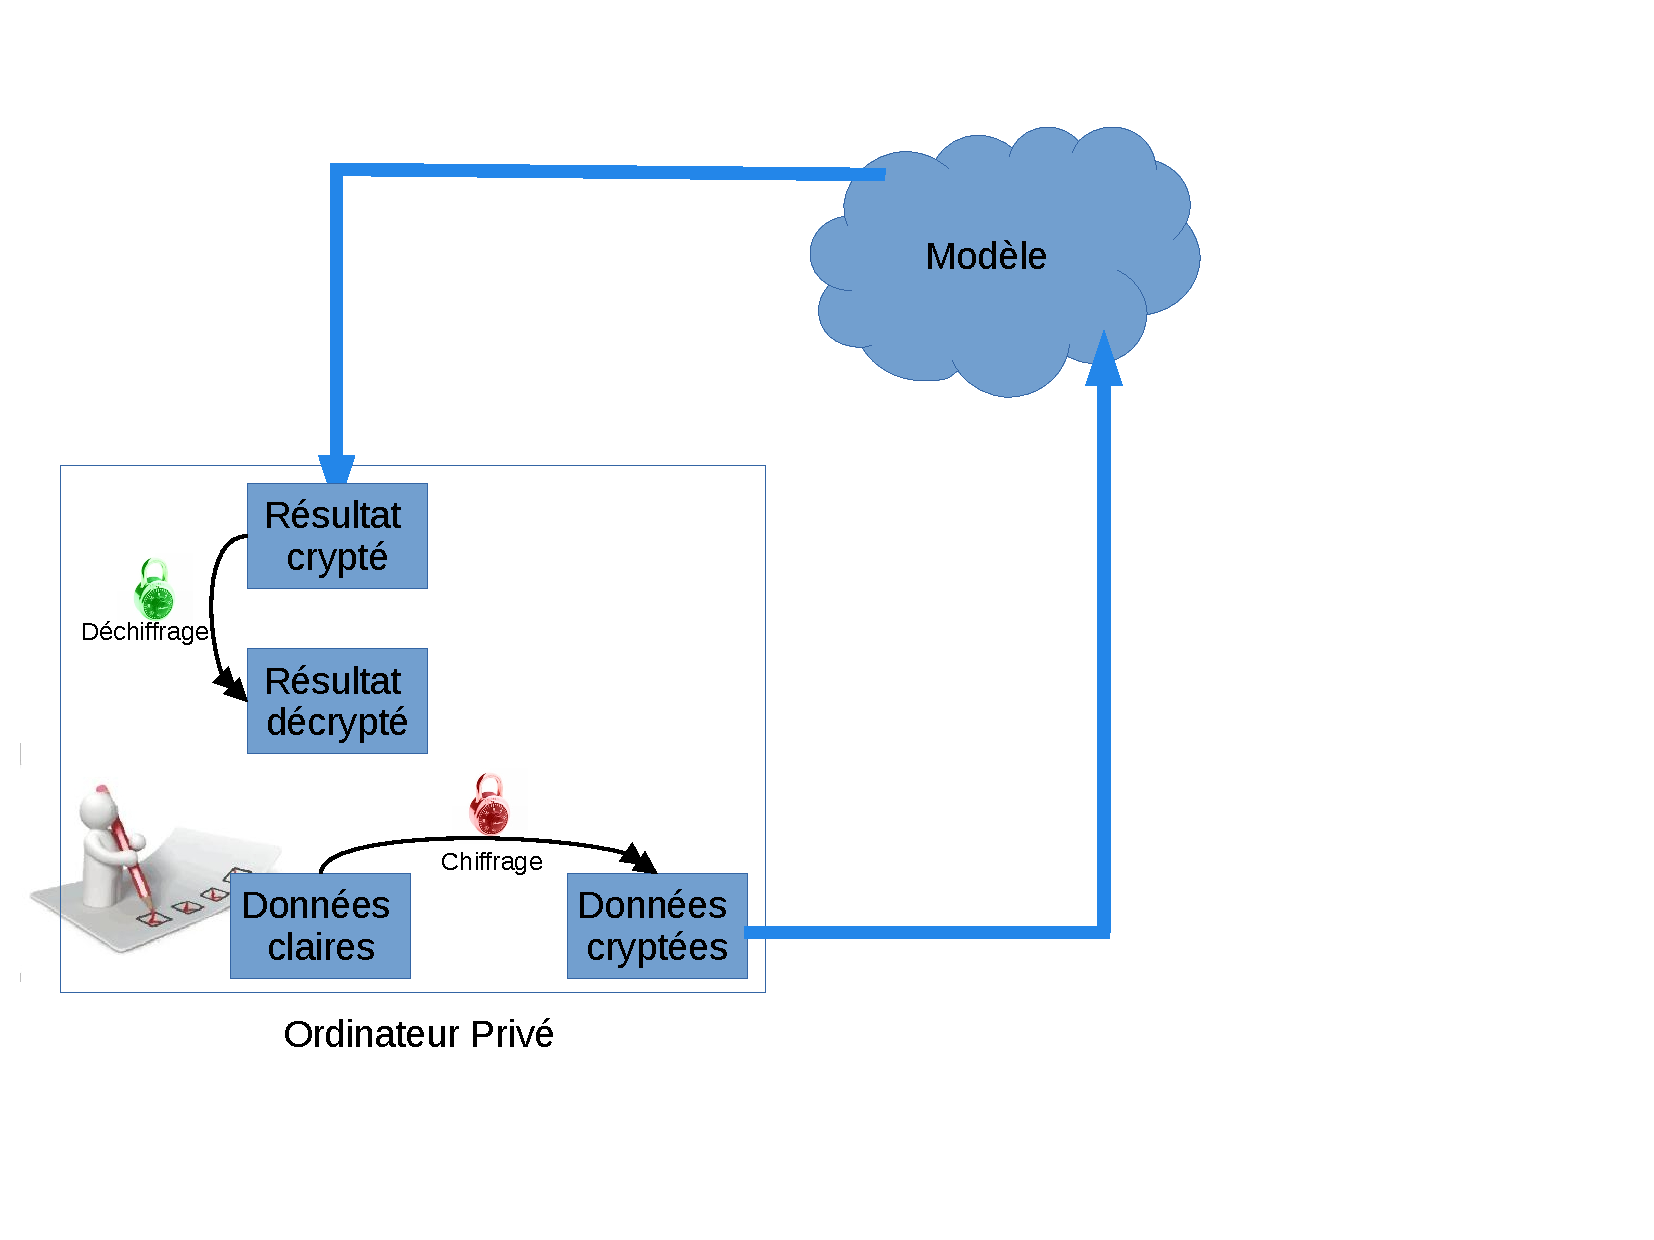
\includegraphics[width=8cm]{SchemaM1.pdf}
            
            \end{center}
        \end{figure}
      }
              }
  \end{itemize}
  \end{frame}
  \begin{frame}{Cryptographie + ML}
  \textbf{\textit{Cryptonets .}}\newline
  \begin{itemize}
    \item{Réseau des neurones.}
    \item{MNIST dataset(chiffres manuscrits).}
    \item{Phase de prédiction avec de données chiffrées.}
    \end{itemize}
\textbf{\textit{Bioinformatics application .}}\newline
  \begin{itemize}
    \item{Régression logistique.}
    \item{Données médicales.}
    \item{Prédiction (Diabète) avec de données chiffrées.}
  \end{itemize}
  \end{frame}
  %////////////SLIDE1\\\\\\\\\\\\\\\\\\
\section{Apprentissage automatique à partir de données chiffrées}
\subsection{Stochastic Gradient Descent(SGD)}
  \begin{frame}{Stochastic Gradient Descent(SGD)}
Descente de gradient stochastique : technique de minimisation de la fonction d'erreur {\tiny appliquable sur toutes fonction differentiables}.\newline

\begin{block}{Algorithme}
\begin{enumerate}
	\item{choisir un point $x_0$.}
	\item{Itérer : 
\begin{itemize}
	\item{Calculer $\nabla f(x_t)$ }
	\item{Mettre à jour $x_{t+1}\leftarrow x_t - \alpha \nabla f(x_t)$}
\end{itemize}
	}
\end{enumerate}
\end{block}
%\begin{figure}[h!]\begin{center}
 %        \includegraphics[width=8cm]{sgd.png}
%\end{center}
%\end{figure}
\end{frame}
%////////////SLIDE1\\\\\\\\\\\\\\\\\\
\subsection{Schéma explicatif}
  \begin{frame}{Schéma explicatif}
  \begin{figure}
   \begin{minipage}[c]{.41\linewidth}
      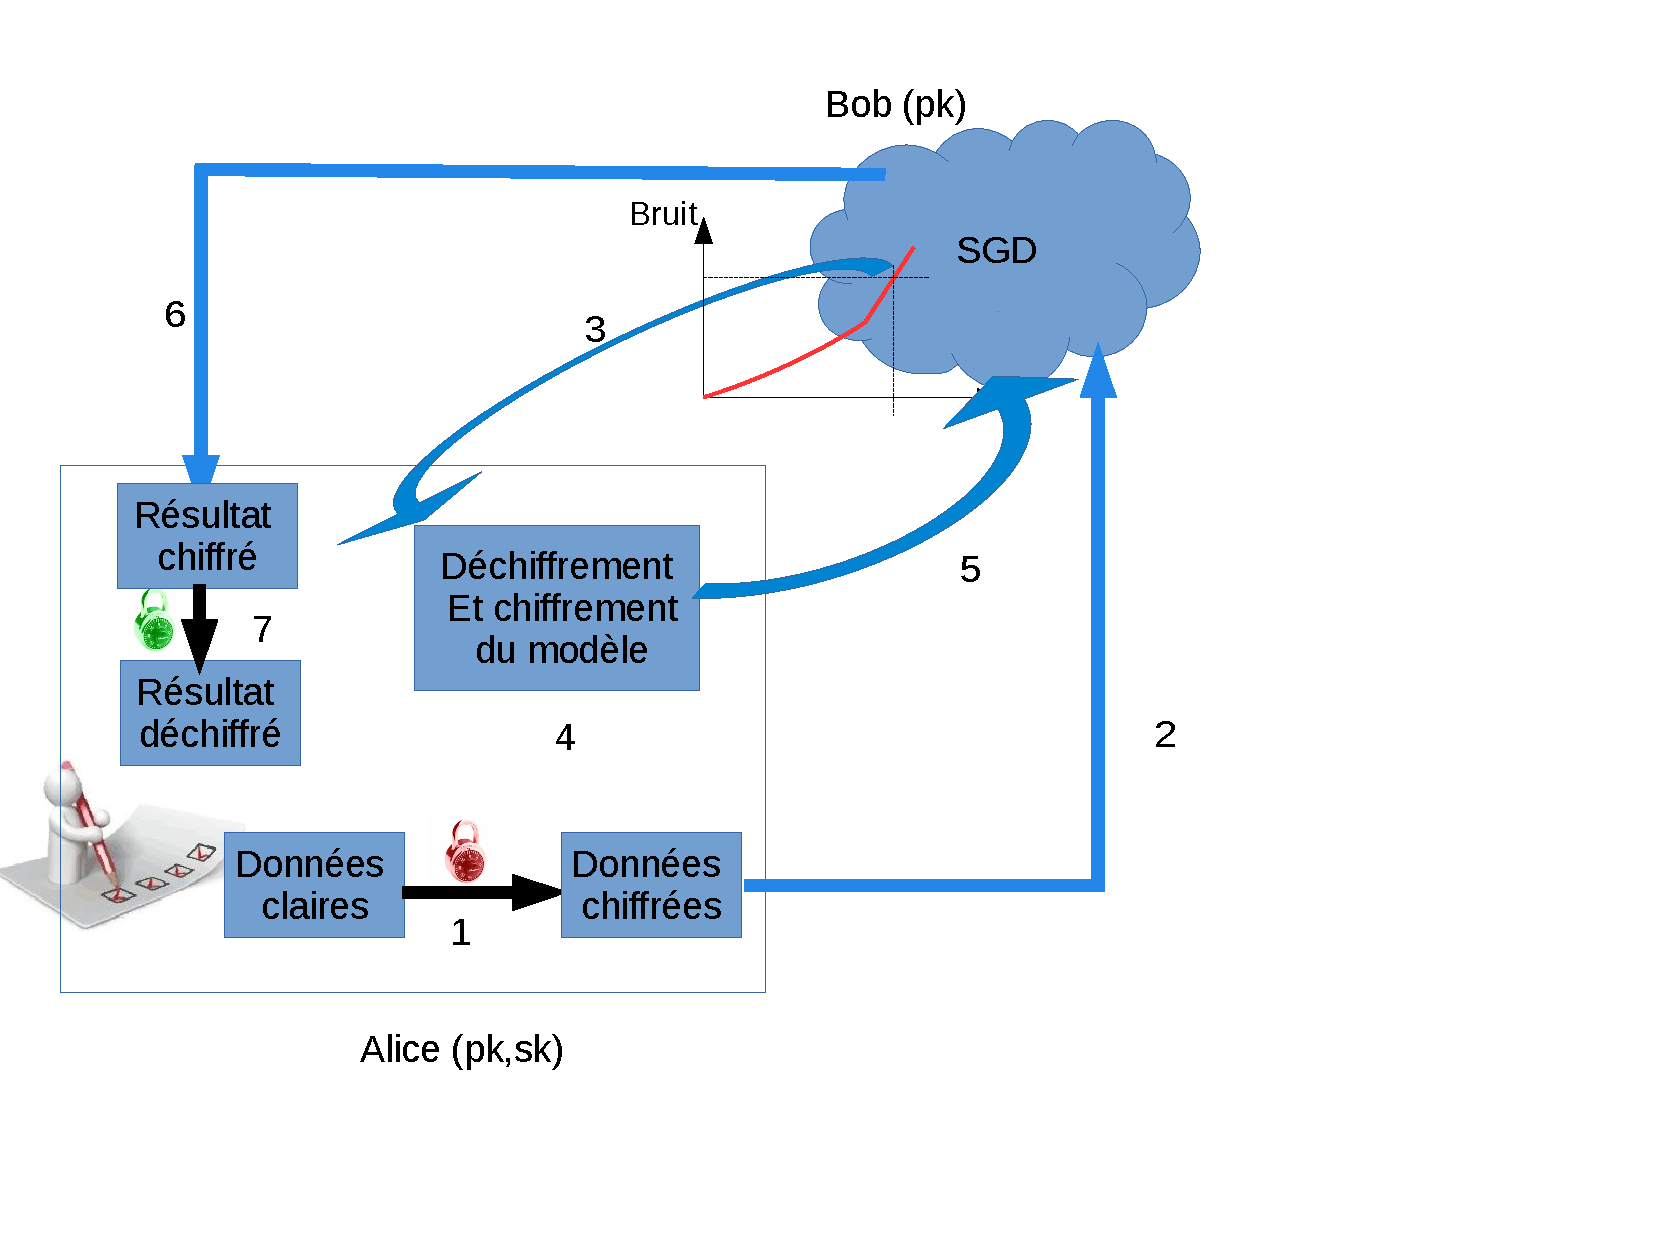
\includegraphics[width=8cm]{SGD_.pdf}
   \end{minipage} \hfill
   \begin{minipage}[c]{.51\linewidth}
      \begin{enumerate}
    		\item {Chiffrement : jeu de données + modèle.}
  			\item {Appliquer SGD sur les données.}
  			\item {Renvoi du modèle à Alice .}
        \item {Alice chiffre et déchiffre le modèle .}
        \item {Renvoi du modèle chiffré à Bob .}
        \item {renvoi du modèle chiffrés.}
        \item {Appliquer la fonction de prédiction.}
		\end{enumerate}
   \end{minipage}
\end{figure}
\end{frame}
%////////////SLIDE1\\\\\\\\\\\\\\\\\\
\subsection{Approximation et résultats}
 \begin{frame}{Approximation et résultats}
 Dans la regression logistique on utilise la fonction sigmoid définie par :\newline
 $$f(x)=\dfrac{1}{1 + exp(-x)}$$
 Comme dans la bibliothèque SEAL la fonction exponentielle n'est pas définie on a dû l'approximer avec :\newline
\begin{enumerate}
	\item{Developpement de Taylor}
	\item{Approximation avec une function linéaire par morceau}
	\item{Fonction carré}
\end{enumerate}
\end{frame}
%////////////SLIDE1\\\\\\\\\\\\\\\\\\
\subsubsection{Developpement de Taylor}
\begin{frame}{Developpement de Taylor}
On a :
\newcommand\omicron{o}
 $$\dfrac{1}{1+e^{-x}} = \dfrac{1}{2} + \dfrac{1}{4}x - \dfrac{1}{48}x^3 + \dfrac{1}{480}x^5 - \dfrac{1}{80640}x^7 + \omicron(x^9)$$
Dans un premier temps on a essayé de faire une approximation avec le developpement de Taylor, sauf qu'avec la fonction puissance (sous le nom exponentiate dans SEAL) on a un bruit qui s'accumule, et le texte chiffré devient vite indéchiffrable. 
\end{frame}
\subsubsection{Approximation avec une function linéaire par morceau}
\begin{frame}{Approximation avec une function linéaire par morceau}
Dans une deuxieme tentative on a approximé la fonction sigmoid avec une fonction linéaire par morceau  qui est définie par :\newline
 \begin{equation}
f(x)=
\left\lbrace
\begin{array}{ccc}
0  & \mbox{si} & x<-2\\
1/2 + x/4 & \mbox{si} & -2<x<2\\
1 & \mbox{si} & x>2
\end{array}\right.
\end{equation}
Avec cette méthode on a réussi a avoir une fonction d'erreur qui converge de la même manière comme si on a travaillé avec des données non chiffrées comme il le montre la figure suivante :
\begin{figure}[h!]\begin{center}
             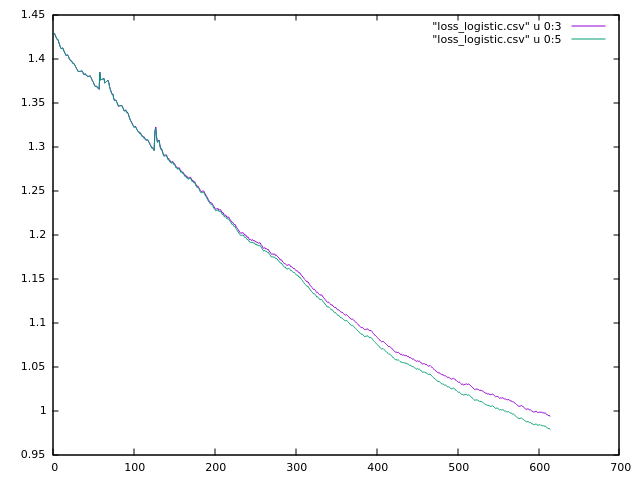
\includegraphics[width=4cm]{loss_logistic_regression.png}
             \end{center}
             \end{figure}
\end{frame}
\subsubsection{Fonction carré}
\begin{frame}{Fonction carré}
\end{frame}
\begin{frame}
	\transdissolve<1>[duration=0.2]
	\begin{center}
	\textcolor{orange}{\textbf{\textit{Merci de votre attention.}}}
	\end{center}
\end{frame}
\end{document}


